\documentclass[
11pt, % The default document font size, options: 10pt, 11pt, 12pt
%codirector, % Uncomment to add a codirector to the title page
]{charter} 

\usepackage{subfig}
\usepackage{lscape}

\usepackage{fontspec}

% El títulos de la memoria, se usa en la carátula y se puede usar el cualquier lugar del documento con el comando \ttitle
\titulo{Visión computacional estereoscópica} 

% Nombre del posgrado, se usa en la carátula y se puede usar el cualquier lugar del documento con el comando \degreename
%\posgrado{Carrera de Especialización en Sistemas Embebidos} 
%\posgrado{Carrera de Especialización en Internet de las Cosas} 
\posgrado{Carrera de Especialización en Inteligencia Artificial}
%\posgrado{Maestría en Sistemas Embebidos} 
%\posgrado{Maestría en Internet de las cosas}

% Tu nombre, se puede usar el cualquier lugar del documento con el comando \authorname
\autor{Ing. Ariel Salassa} 

% El nombre del director y co-director, se puede usar el cualquier lugar del documento con el comando \supname y \cosupname y \pertesupname y \pertecosupname
\director{Esp. Ing. Hernán Contigiani}
\pertenenciaDirector{Globant} 
% FIXME:NO IMPLEMENTADO EL CODIRECTOR ni su pertenencia
\codirector{John Doe} % para que aparezca en la portada se debe descomentar la opción codirector en el documentclass
\pertenenciaCoDirector{FIUBA}

% Nombre del cliente, quien va a aprobar los resultados del proyecto, se puede usar con el comando \clientename y \empclientename
\cliente{Esp. Ing. Hernán Contigiani}
\empresaCliente{Globan}

% Nombre y pertenencia de los jurados, se pueden usar el cualquier lugar del documento con el comando \jurunoname, \jurdosname y \jurtresname y \perteunoname, \pertedosname y \pertetresname.
\juradoUno{Nombre y Apellido (1)}
\pertenenciaJurUno{pertenencia (1)} 
\juradoDos{Nombre y Apellido (2)}
\pertenenciaJurDos{pertenencia (2)}
\juradoTres{Nombre y Apellido (3)}
\pertenenciaJurTres{pertenencia (3)}
 
\fechaINICIO{26 de abril de 2022}		%Fecha de inicio de la cursada de GdP \fechaInicioName
\fechaFINALPlan{14 de junio de 2022} 	%Fecha de final de cursada de GdP
\fechaFINALTrabajo{diciembre de 2022}	%Fecha de defensa pública del trabajo final


\begin{document}

\maketitle
\thispagestyle{empty}
\pagebreak


\thispagestyle{empty}
{\setlength{\parskip}{0pt}
\tableofcontents{}
}
\pagebreak


\section*{Registros de cambios}
\label{sec:registro}


\begin{table}[ht]
\label{tab:registro}
\centering
\begin{tabularx}{\linewidth}{@{}|c|X|c|@{}}
\hline
\rowcolor[HTML]{C0C0C0} 
Revisión & \multicolumn{1}{c|}{\cellcolor[HTML]{C0C0C0}Detalles de los cambios realizados} & Fecha      \\ \hline
0.0      & Creación del documento                                 			& 26/04/2022 \\ \hline
1.0      & Se completa hasta la sección 5 inclusive               	& 08/05/2022 \\ \hline

1.1      & Correcciones de la versión 1.0                 					& 20/05/2022 \\ \hline
2.0      & Se completa hasta la sección 9 inclusive					& 22/05/2022 \\ \hline
2.1      & Correcciones de la versión 2.0					& 26/05/2022 \\ \hline
3.0      & Se completa hasta sección 12 inclusive					& 29/05/2022 \\ \hline
3.1      & Correcciones de la versión 3.0					& 03/06/2022 \\ \hline
4.0      & Se completa hasta sección 12 inclusive					& 04/06/2022 \\ \hline
4.1      & Correcciones de la versión 4.0					& 06/06/2022 \\ \hline
%		  Se puede agregar algo más \newline
%		  En distintas líneas \newline
%		  Así                                                    & dd/mm/aaaa \\ \hline
%3      & Se completa hasta el punto 11 inclusive                & dd/mm/aaaa \\ \hline
%4      & Se completa el plan	                                 & dd/mm/aaaa \\ \hline
\end{tabularx}
\end{table}

\pagebreak



\section*{Acta de constitución del proyecto}
\label{sec:acta}

\begin{flushright}
Buenos Aires, \fechaInicioName
\end{flushright}

\vspace{2cm}

Por medio de la presente se acuerda con el \authorname\hspace{1px} que su Trabajo Final de la \degreename\hspace{1px} se titulará ``\ttitle'' y  consistirá en investigar el estado del arte de la visón computacional realizada con más de una cámara como entrada, de modo que se puedan tomar decisiones en un ambiente 3D simulado, con fecha de inicio \fechaInicioName\hspace{1px} y fecha de presentación pública \fechaFinalName. Se estima que el valor aproximado del proyecto es de \emph{15405 USD} y que tendrá una duración de 588 hs aproximadamente.

Se adjunta a esta acta la planificación inicial.

\vfill

% Esta parte se construye sola con la información que hayan cargado en el preámbulo del documento y no debe modificarla
\begin{table}[ht]
\centering
\begin{tabular}{ccc}
\begin{tabular}[c]{@{}c@{}}Ariel Lutenberg \\ Director posgrado FIUBA\end{tabular} & \hspace{2cm} & \begin{tabular}[c]{@{}c@{}}\clientename \\ \empclientename \end{tabular} \vspace{2.5cm} \\ 
\multicolumn{3}{c}{\begin{tabular}[c]{@{}c@{}} \supname \\ Director del Trabajo Final\end{tabular}} \vspace{2.5cm} \\
%\begin{tabular}[c]{@{}c@{}}\jurunoname \\ Jurado del Trabajo Final\end{tabular}     &  & \begin{tabular}[c]{@{}c@{}}\jurdosname\\ Jurado del Trabajo Final\end{tabular}  \vspace{2.5cm}  \\
%\multicolumn{3}{c}{\begin{tabular}[c]{@{}c@{}} \jurtresname\\ Jurado del Trabajo Final\end{tabular}} \vspace{.5cm}                                                                     
\end{tabular}
\end{table}




\section{1. Descripción técnica-conceptual del proyecto a realizar}
\label{sec:descripcion}

La visión computacional en pocas palabras consta de cámaras que entregan fotogramas a un sistema que los toma y los procesa teniendo en cuenta
una calibración previa.

La idea del proyecto se basa en el uso de al menos dos cámaras conectadas a un mismo sistema de visión que sea capaz de procesar las imágenes de cada una de las cámaras permitiendo estimar atributos de objetos tales como altura, profundidad y volumen. 

Actualmente existen cámaras estereoscópicas integradas en un único dispositivo (Figura \ref{fig:camera}) que realizan dichas tareas, permitiendo agregar funcionalidades como la navegación de robots o asistencia a conductores. Las cámaras estereoscópicas integradas tienen la ventaja de que el mismo hardware y firmware realiza la inferencia, pero tienen la desventaja de que la distancia entre cámaras es fija y esto no permite tomar espectros 3D en infraestructuras preexistentes. 

\begin{figure}[H]
\centering
\frame{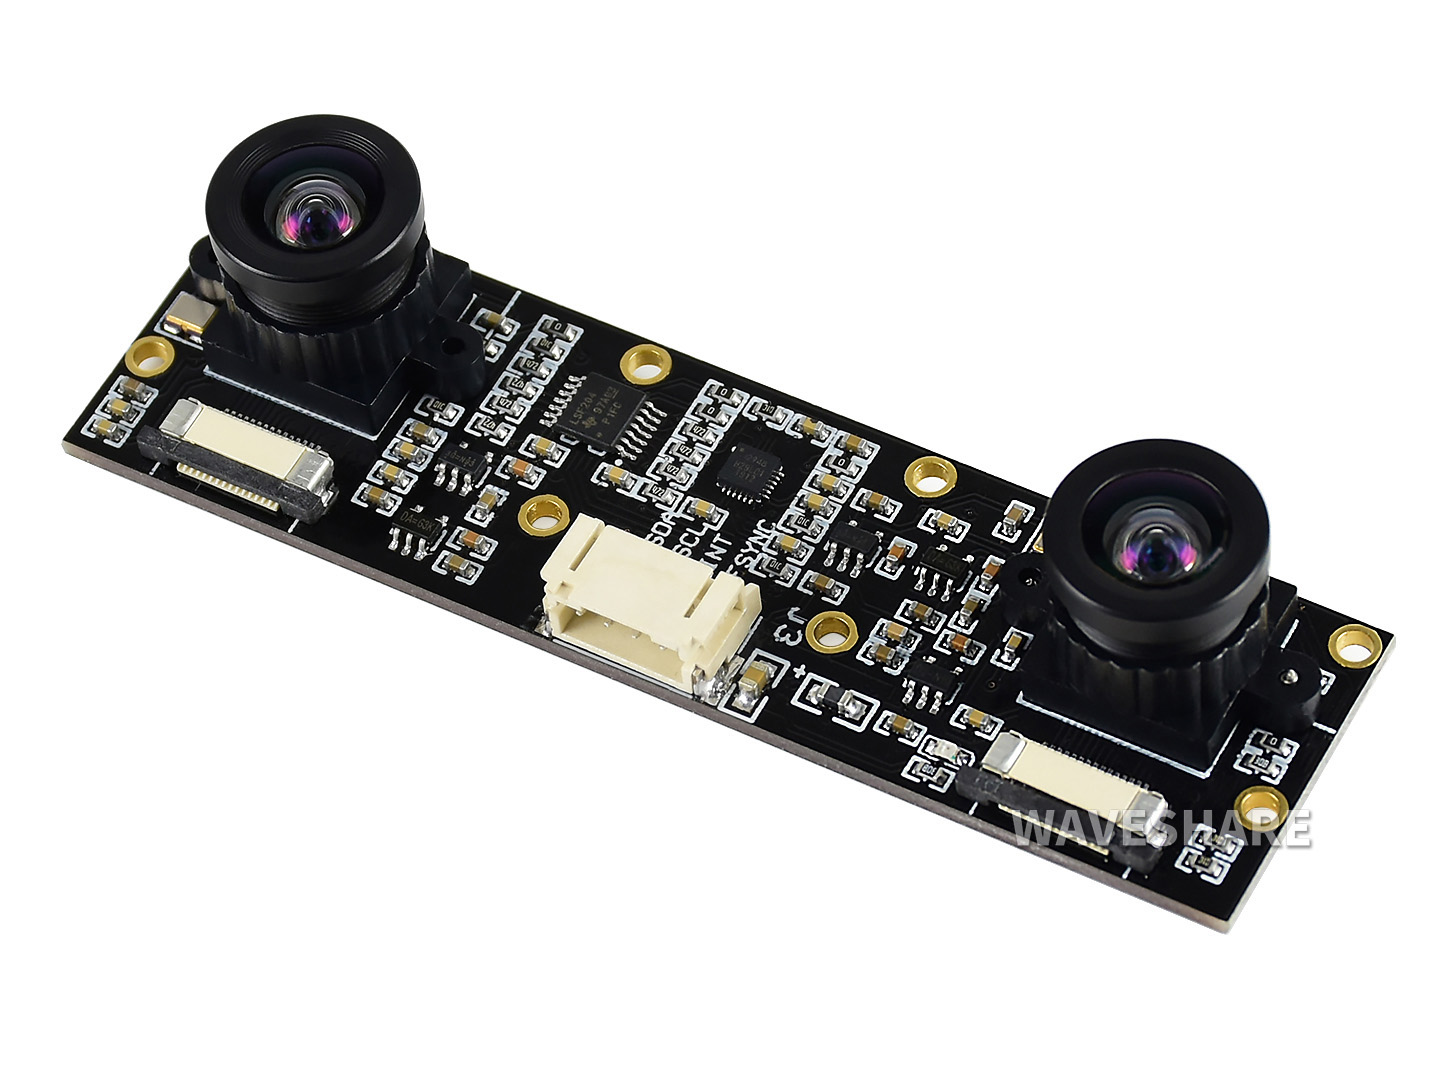
\includegraphics[width=.5\textwidth]{./Figuras/stereo_camera.jpg}}
\caption{Cámara estereoscópica.}
\label{fig:camera}
\end{figure}

Tener un sistema de cámaras conectado a un servidor puede otorgar mucha más precisión como así también, mejor alcance de la solución. Incluso se podría evaluar la posibildad de hacer visión computacional estereoscópica con cámaras que no están fijas.

Las partes que conforman un sistema de visión computacional se pueden observar en el siguiente diagrama de la Figura \ref{fig:system}.

\begin{figure}[H]
\centering
\frame{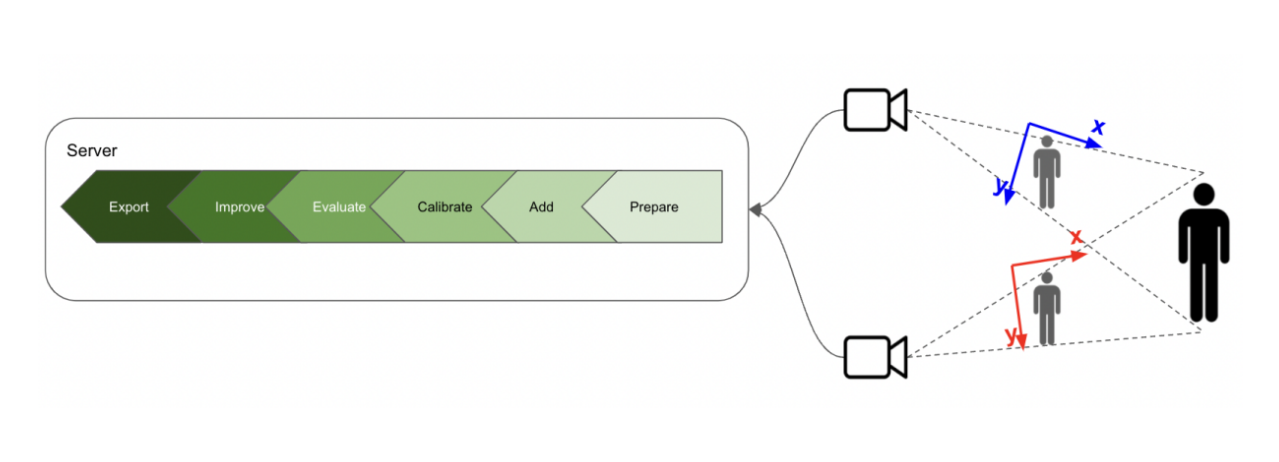
\includegraphics[width=.9\textwidth]{./Figuras/vision_system.png}}
\caption{Partes de un sistema de visión computacional.}
\label{fig:system}
\end{figure}


\section{2. Identificación y análisis de los interesados}
\label{sec:interesados}

\begin{table}[ht]
\begin{tabularx}{\linewidth}{@{}|l|X|l|X|@{}}
\hline
\rowcolor[HTML]{C0C0C0} 
Rol           & Nombre y Apellido & Organización 	& Puesto 	\\ \hline
Responsable   & \authorname       & Autónomo   & Sr. Software Engineer \newline Alumno 	\\ \hline
Cliente & Ing. Juan Pablo Pizarro 
    						& Globant  
    						& Software Development Specialist \newline 
    							\\ \hline
Orientador    & \supname	      & \pertesupname 	& Sr. Software Engineer \newline Director Trabajo final \\ \hline
Usuario final & Desarrolladores de Software & -   & Software developers       	\\ \hline
\end{tabularx}
\caption{Identificación de los interesados.}
\label{tab:interesados}
\end{table}

\begin{itemize}
	\item Responsable: \authorname, es la persona que desarrollará el proyecto.
	\item Cliente: El Ing. Juan Pablo Pizarro, es líder y referente técnico del equipo de desarrollo del departamento de IOT de Globant. Él es el principal interesado en que su departamento cuente con alguna solución de visión esteoscópica. Por sus altos grados de conocimientos ténicos también puese ser capaz de orientar en el desarrollo.
	\item Orientador: Hernán Contigiani es el director del presente proyecto y líder técnico en Globant. Su función será orientar al responsable a lo largo de la realización del proyecto.
	\item Desarrolladores de Software: son los usuarios finales que podrán hacer uso del sistema para enriquecer sus aplicaciones.
\end{itemize}

\section{3. Propósito del proyecto}
\label{sec:proposito}
El propósito del proyecto es investigar el estado del arte de la visión computacional con más de una cámara como entrada de video de modo de que se puedan tomar decisiones en un ambiente 3D simulado. Con ello se pretende llegar a un sistema de visón estereoscópica más versátil que aquellos integrados en un dispositivo.

\section{4. Alcance del proyecto}
\label{sec:alcance}
El proyecto comprenderá las siguientes etapas:
\begin{itemize}
\item Planificación de tareas.
\item Formación en visión computacional.
\item Investigación de sistemas utilizados en cámaras estereoscópicas.
\item Formación en protocolos de comunicación utilizados para \emph{straming}.
\item Configuración y calibración de cámaras.
\item Comunicacion remota entre las cámaras y el servidor.
\item Preparación de los datos.
\item Extracción de características.
\item Prototipado conceptual funcional.
\item Reporte de resultados.
\end{itemize}


El presente proyecto no incluye:
\begin{itemize}
\item Desarrollo fino de redes neuronales que permitan detectar y clasificar objetos.
\end{itemize}


\section{5. Supuestos del proyecto}
\label{sec:supuestos}
Para el desarrollo del presente proyecto se supone que:
\begin{itemize}
	\item El responsable dispondrá de suficiente cantidad de tiempo para resolver los problemas que se presenten en el desarrollo del proyecto.
	\item El responsable tendrá a su disposición a su director y/o colaboradores cuando sea pertinente.
	\item Se puede alcanzar un prototipo del sistema utilizando \emph{webcams}.
	\item Se dispondrá de suficiente potencia de cómputo para trabajar con \emph{straming} de imágenes.
	\item Es posible realizar una composición de dos o más imágenes en una única imagen de salida que permita estimar profundidad y volumen de los objetos presentes en la imagen. 
	\item Se puede aplicar el protocolo RTMP (\emph{Real Time Messaging Protocol}) o RTSP (\emph{Real Time Streaming Protocol}) para la adquisión remota de las imágenes.
	\item Se puede integrar al sistema una red neuronal pre entrenada para detectar objetos.
\end{itemize}

\section{6. Requerimientos}
\label{sec:requerimientos}

\begin{enumerate}
	\item Requerimientos de documentación
		\begin{enumerate}
			\item El trabajo debe ser continuamente documentado y se presentarán informes mesnsuales de avance al director.
			\item Los informes de avance pueden ser presentados como código correctamente documentado con los resultados correspondientes.
			\item El código final será de tipo abierto y deberá quedar ordenado en un repositorio público.
		\end{enumerate}
	\item Requerimientos de lenguajes y frameworks
		\begin{enumerate}
			\item La biblioteca para el tratamiento de las imágenes será \emph{OpenCV}.
			\item El código para el desarrollo deberá ser escrito en Python. Si se requiriese una optimización de hardware, entonces deberá utilizarse C++.
			\item Se deberá priorizar el uso de bibliotecas estándar  (NumPy, Pandas, Matplotlib, Seaborn, etcétera).
		\end{enumerate}
	\item Requerimientos funcionales
		\begin{enumerate}
			\item El sistema de visión debe estar compuesto por al menos dos cámaras.
			\item Cada cámara debe estar correctamente calibrada.
			\item El sistema de visión debe poder comandarse de manera remota.
			\item La transmisión de imágenes desde el sistema de visión hacia el resto del sistema de clasificación y evaluación debe hacerse usando protocolos de transmisión en tiempo real.
			\item El sistema debe ser capaz de detectar objetos y determinar profundidad, volumen y/o distancia de los mismos.
			\item El error del sistema no deberá ser superior al 15 \%.
		\end{enumerate}
	\item Requerimientos de testing y evaluación
		\begin{enumerate}
			\item Los resultados del sistema deberán ser corroborados previamente en un entorno local y con objetos de dimesiones conocidas.
		\end{enumerate}
\end{enumerate}

\section{7. Historias de usuarios (\textit{Product backlog})}
\label{sec:backlog}
La medida del trabajo a efectuar para cumplir con cada una de las historias de usuarios estará dada por \emph{story points}. Para ponderar los esfuerzos se utilizará la serie de Fibonacci con valores: 0, 1, 2, 3, 5, 8, 13, 21, 34, 55, 89, etc. Cuando el esfuerzo se considere alto los \emph{story points} tomarán valores entre 0 y 3 inclusive. Cuando se considere medio, entre 5 y 13 inclusive. Cuando el esfuerzo se considere alto el valor de los \emph{story points} será igual o mayor a 21.

\begin{itemize}
\item Como desarrollador quiero un prototipo de visión esteroscópica que pueda extraer caracterísitcas como distancia, profundidad y volúmen de objectos. 

Dificultad: alta (34) -- Complejidad: alta (34)  -- Incertidumbre: alta (34)

Story Points: 34 + 34 + 34 = 102 $\rightarrow$ 89

\item Como cliente quiero tener un sistema de visón realizado con tecnologías estándar y \emph{open source} para poder mantenerlo a futuro con el menor esfuerzo posible.

Dificultad: media (8) -- Complejidad: media (8) -- Incertidumbre: baja (1)

Story Points: 8 + 8 + 1 = 17 $\rightarrow$ 21

\item Como desarrollador quiero poder acceder remotamente al sistema de visión.

Dificultad: alta (21)  -- Complejidad: alta (21) -- Incertidumbre: alta (21)

Story Points: 21 + 21 + 21 = 63 $\rightarrow$  55

\item Como cliente quiero tener el prototipo de un sistema de visión que permita futuras iteraciones.

Dificultad: media (8) -- Complejidad: media (8) -- Incertidumbre: alta (21)

Story Points: 8 + 8 + 21 = 37 $\rightarrow$ 34

\item Como cliente quiero recibir la documentación del trabajo realizado para que pueda servir como base de futuros desarrollos de la empresa.

Dificultad: media (13) -- Complejidad: baja (2) -- Incertidumbre: baja (1)

Story Points: 13 + 2 + 1 = 16 $\rightarrow$ 13

\item Como cliente quiero tener una presentación resumida del trabajo para mostrar sus resultados y su potencial potencial a todos los interesados.

Dificultad: baja (3) -- Complejidad: baja (2) -- Incertidumbre: baja (2)

Story Points: 3 + 2 + 2 = 7 $\rightarrow$ 8


\end{itemize}

\section{8. Entregables principales del proyecto}
\label{sec:entregables}

Los entregables del proyecto son:

\begin{itemize}
 \item Informe final.
 \item Presentación final.
 \item Diagrama de funcionamiento.
 \item Prototipo conceptual funcional.
 \item Repositorio de código del sistema.
 \item Informe de avance.
\end{itemize}

\section{9. Desglose del trabajo en tareas}
\label{sec:wbs}


\begin{enumerate}
\item Planificación. (60 hs)
	\begin{enumerate}
		\item Estudio de necesidades. (9 hs)
		\item Análisis de factibilidad. (3 hs)
		\item Definición de requerimientos. (9 hs)
		\item Confección de documento de planificación. (39 hs)
	\end{enumerate}
\item Investigación y capacitación. (114 hs)
	\begin{enumerate}
		\item Capacitación en conceptos básicos de visión esteroscópica y sus aplicaciones. (9 hs)
		\item Capacitación en geometría de la formación de imágenes. (6 hs)
		\item Capacitación en geometría epipolar. (6 hs)
		\item Capacitación en distorsión de lentes. (6 hs)
		\item Capacitación en calibración de cámaras. (6 hs)
		\item Capacitación en \emph{OpenCV}. (21 hs)
		\item Capacitación en protocolos de \emph{streaming} en tiempo real. (15 hs)
		\item Elaboración de código de ejemplo de visión estereoscópica. (30 hs)
		\item Elaboración de código de ejemplo de uso de protocolos en tiempo real. (15 hs)
	\end{enumerate}
\item \emph{Setup} de cámaras. (45 hs)
	\begin{enumerate}
		\item Conexión de cámaras y acceso al \emph{stream} de video mediante ordenador. (15 hs)
		\item Calibración de cámaras individuales. (15 hs)
		\item Montaje de cámaras y calibración conjunta. (15 hs)
	\end{enumerate}
\item Construcción del \emph{pipeline} de preparación de datos. (51 hs)
	\begin{enumerate}
		\item Suavizado y ajuste de tamaño. (15 hs)
		\item Filtro de distorsión de lentes. (21 hs)
		\item Evaluación y selección de FPS \emph{(frames per second)} del sistema. (15 hs)
	\end{enumerate}
\item Evaluación estéreo. (105 hs)
	\begin{enumerate}
 		\item Detección de objectos de cada imagen. (15 hs)
 		\item Implementación de \emph{template matching}. (15 hs)
 		\item Implementación de geometría epipolar. (15 hs)
 		\item Implementación de disparidad estéreo. (15 hs)
 		\item Cálculo de distacias y profundidades. (15 hs)
 		\item Estimación volumétrica. (15hs)
 		\item Prototipado y preparación de resultados de salida. (15 hs)
 	\end{enumerate}
\item Pruebas de validación. (63 hs)
	\begin{enumerate}
		\item Pruebas locales en tiempo real. (21 hs)
		\item Pruebas remotas en tiempo real. (21 hs)
		\item Ajustes finales. (21 hs)
	\end{enumerate}

\item Documentación y presentación final. (150 hs)
 	\begin{enumerate}
 		\item Elaborar informe de avance proyecto. (39 hs)
 		\item Elaborar informe final del proyecto. (90 hs)
 		\begin{enumerate}
			\item Redacción y corrección capítulo I. (18 hs)
			\item Redacción y corrección capítulo II. (18 hs)
			\item Redacción y corrección capítulo III. (18 hs)
			\item Redacción y corrección capítulo IV. (18 hs)
			\item Redacción y corrección capítulo V. (18 hs)
		\end{enumerate}
 		\item Preparación de presentación final. (21 hs)
 	\end{enumerate}
\end{enumerate}

Cantidad total de horas: (588 hs)

\section{10. Diagrama de Activity On Node}
\label{sec:AoN}

En la Figura \ref{fig:aon} se muestra el diagrama de \emph{Activity on Node} del proyecto. Las flechas resaltadas en negro ilustran el camino crítico del proyecto. También se puede ver que los hitos marcan el fin de las distintas fases del proyecto que, a su vez, están representadas en distintos colores. 

La primera fase está comprendida por tareas previas al desarrollo en código del proyecto. En esta fase se considera la planificación y la capacitación.

La segunda fase involucra todo el \emph{pipeline} necesario para tratar las imágenes y obtener resultados de salida.

La tercera fase consiste en tomar como punto de partida un sistema ya prototipado para someterlo a distintas pruebas de interés.

Finalmente, la última fase, involucra toda la realización de toda la documentación del trabajo realizado.

\begin{figure}[htpb]
\centering 
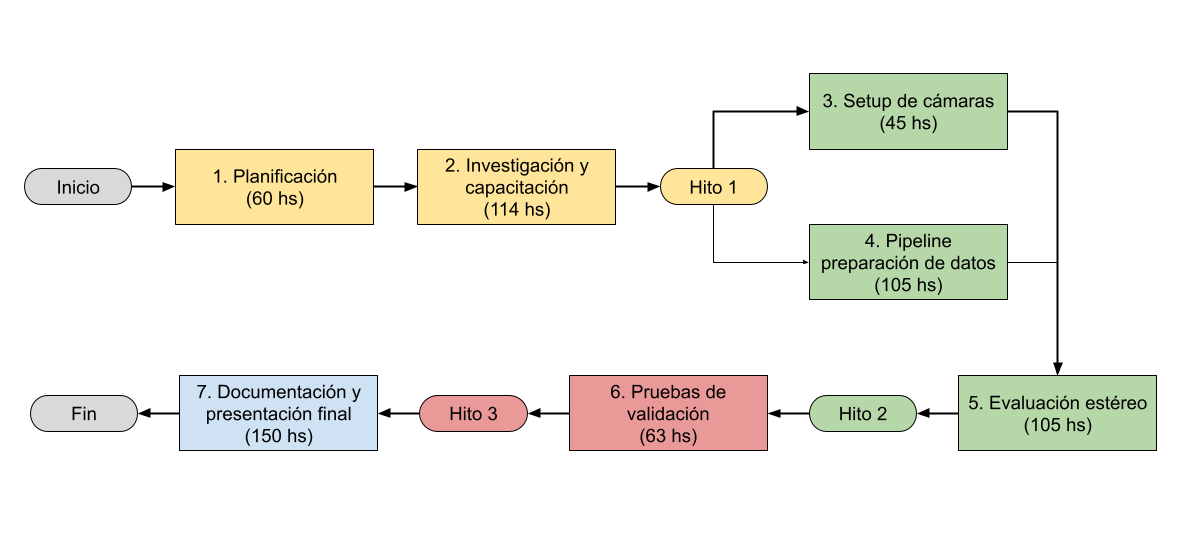
\includegraphics[width=\textwidth]{./Figuras/aon.png}
\caption{Diagrama en \textit{Activity on Node.}}
\label{fig:aon}
\end{figure}

\section{11. Diagrama de Gantt}
\label{sec:gantt}

A continuación se muestra el diagrama de Gant del presente proyecto. Se consideró la jornada laboral de 3 horas de trabajo desde la fecha de inicio del curso hasta finales de año.
En la figura \ref{fig:gantt} se muestra el diagrama de Gantt, tal como se enumeró en la sección 9.

\begin{landscape}
\begin{figure}[htpb]
\centering 
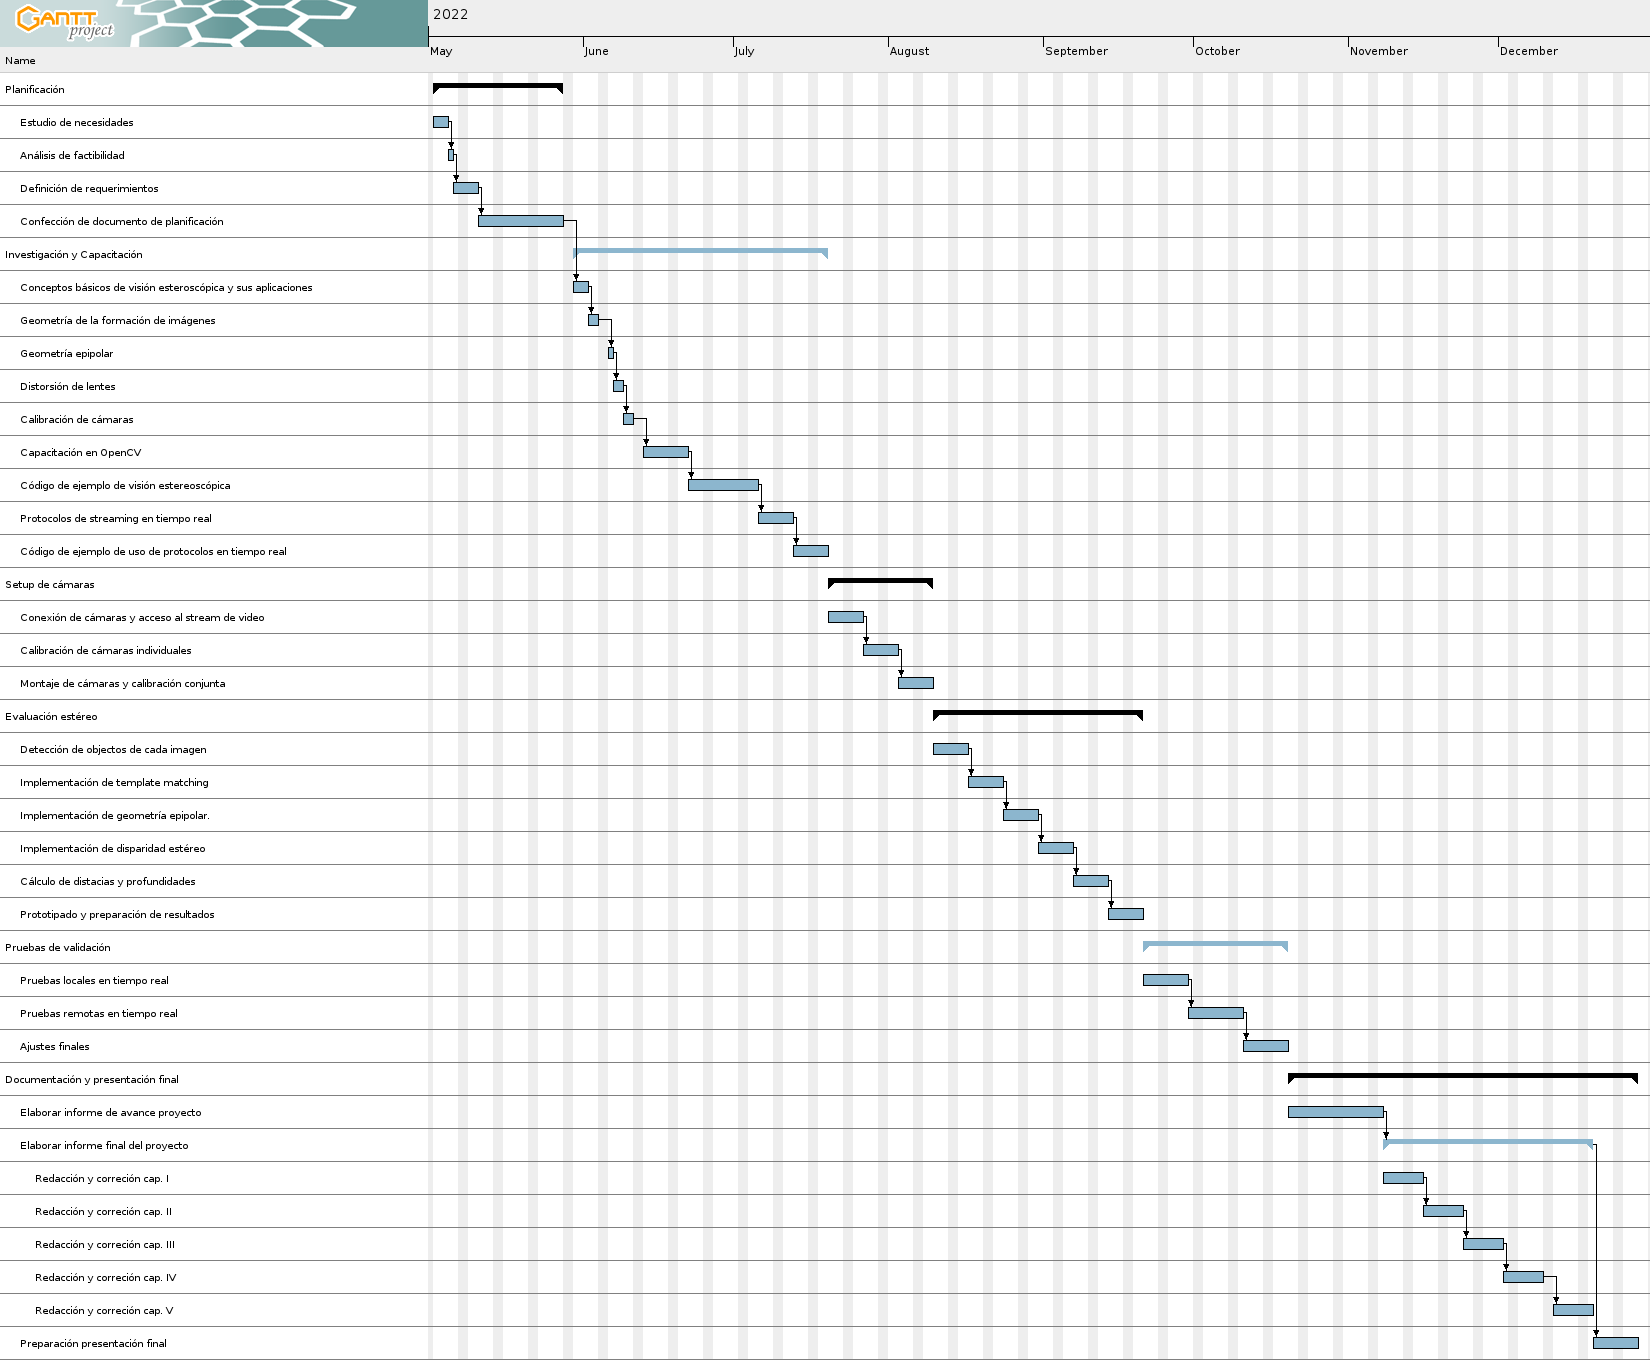
\includegraphics[width=24cm, height=15cm]{./Figuras/gantt.png}
\caption{Diagrama de Gantt.}
\label{fig:gantt}
\end{figure}
\end{landscape}

\section{12. Presupuesto detallado del proyecto}
\label{sec:presupuesto}

En esta sección se detallan los gastos del proyecto. Las unidades del valor unitario están dadas en dólares estadounidenses. Al momento de redactar este informe la cotización oficial es de $1 USD = 121 ARS$.

\begin{table}[htpb]
\centering
\begin{tabularx}{\linewidth}{@{}|X|c|r|r|@{}}
\hline
\rowcolor[HTML]{C0C0C0} 
\multicolumn{4}{|c|}{\cellcolor[HTML]{C0C0C0}COSTOS DIRECTOS} \\ \hline
\rowcolor[HTML]{C0C0C0} 
Descripción &
  \multicolumn{1}{c|}{\cellcolor[HTML]{C0C0C0}Cantidad} &
  \multicolumn{1}{c|}{\cellcolor[HTML]{C0C0C0}Valor unitario} &
  \multicolumn{1}{c|}{\cellcolor[HTML]{C0C0C0}Valor total [USD]} \\ \hline
 	Mano de obra & 
  	\multicolumn{1}{c|}{590 horas} &
  	\multicolumn{1}{c|}{20 USD/hora} &
  	\multicolumn{1}{c|}{11800} \\ \hline
 	WebCam &
  	\multicolumn{1}{c|}{2 unidades} &
  	\multicolumn{1}{c|}{25 USD} &
  	\multicolumn{1}{c|}{50} \\ \hline
\multicolumn{3}{|c|}{SUBTOTAL} &
  \multicolumn{1}{c|}{11850} \\ \hline
\rowcolor[HTML]{C0C0C0} 
\multicolumn{4}{|c|}{\cellcolor[HTML]{C0C0C0}COSTOS INDIRECTOS} \\ \hline
\rowcolor[HTML]{C0C0C0} 
Descripción &
  \multicolumn{1}{c|}{\cellcolor[HTML]{C0C0C0}Cantidad} &
  \multicolumn{1}{c|}{\cellcolor[HTML]{C0C0C0}Valor unitario} &
  \multicolumn{1}{c|}{\cellcolor[HTML]{C0C0C0}Valor total [USD]} \\ \hline
	30\% del costo directo & 
  	\multicolumn{1}{c|}{-} &
  	\multicolumn{1}{c|}{-} &
  	\multicolumn{1}{c|}{3555} \\ \hline
\multicolumn{3}{|c|}{SUBTOTAL} &
  \multicolumn{1}{c|}{3555} \\ \hline
\rowcolor[HTML]{C0C0C0}
\multicolumn{3}{|c|}{TOTAL} &
   \multicolumn{1}{c|}{15405} \\ \hline
\end{tabularx}%
\end{table}

\section{13. Gestión de riesgos}
\label{sec:riesgos}

a) Identificación de los riesgos del proyecto:

Riesgo 1: falta de tiempo del responsable.
\begin{itemize}
	\item Severidad (5): se atrasarían las tareas, no se cumpliría con la planificación y, en el peor de los casos, no se lograría completar el proyecto para la fecha de presentación establecida.
	\item Probabilidad de ocurrencia (5): el responsable no trabaja en la misma empresa que ha propuesto el proyecto y, lógicamente, el trabajo es ponderante sobre el proyecto. 
\end{itemize}   

Riesgo 2: no contar con suficiente capacidad de cómputo.
\begin{itemize}
	\item Severidad (8): trabajar con procesamiento de imágenes siempre consume una parte considerable de los recursos de hardware. No contar con el equipo adecuado implicaría que las tareas se harían más largas de lo estimado o que se deberían contratar servicios en la nube que encarecerían el costo del proyecto.
	\item Probabilidad de ocurrencia (2): el responsable posee un equipo adecuado y posee un equipo aceptable de \emph{back up} ante cualquier eventualidad. 
\end{itemize}

Riesgo 3: no contar con las cámaras necesarias. 
\begin{itemize}
	\item Severidad (7): toda prueba debería ser en base a dispositivos simulados que no suelen encontrarse fácilmente. El mero hecho de buscar un dispositivo sería una tarea imprevista que alargaría los tiempos del proyecto.
	\item Probabilidad de ocurrencia (3): la oferta de cámaras de calidad aceptable es amplia. 
\end{itemize}

Riesgo 4: mala calibración de cámaras.
\begin{itemize}
	\item Severidad (6): la correcta calibración de las cámaras es un requerimiento para las etapas posteriores del proyecto. Una mala calibración impediría el avance del proyecto y, por lo tanto, alargaría los tiempos estimados.
	\item Probabilidad de ocurrencia (4): la calibración es un proceso iterativo donde se usan patrones definidos por el desarrollador. Hay una serie de posibles errores sistemáticos en el proceso que podrían causar problemas. 
\end{itemize}

Riesgo 5: comportamiento inesperado del sistema a la hora de evaluar disparidad. 
\begin{itemize}
	\item Severidad (8): el riesgo implicaría adentrarse en profundidad en el comportamiento de la cámara seleccionada, en la implentación de código de \emph{OpenCV} o volver al paso de calibración, dilatando considerablemente los tiempos. Además, sin un correcto mapa de disparidad, nunca se podría estimar la distancia de un objeto a las cámaras o el volumen de un objeto detectado.
	\item Probabilidad de ocurrencia (3): la biblioteca seleccionada es conocida por su robustez y una buena calibración debería evitar este riesgo.
\end{itemize}


b) Tabla de gestión de riesgos:      (El RPN se calcula como RPN=SxO)

\begin{table}[htpb]
\centering
\begin{tabularx}{\linewidth}{@{}|X|c|c|c|c|c|c|@{}}
\hline
\rowcolor[HTML]{C0C0C0} 
Riesgo & S & O & RPN & S* & O* & RPN* \\ \hline
       Falta de tiempo del responsable & 5  & 4  & 20 & - & - & 20 \\ \hline
       No contar con suficiente capacidad de cómputo & 8  & 2  & 16 & - & - & 16     \\ \hline
       No contar con las cámaras necesarias & 7  & 3 & 21 &  -  &  -  &  21    \\ \hline
       Mala calibración de cámaras & 6 & 4 & 24 & 4 & 1 & 4     \\ \hline
      Comportamiento inesperado del sistema a la hora de evaluar disparidad & 8 & 3 & 24 & 5  & 1   & 5  \\ \hline
\end{tabularx}
\end{table}

Criterio adoptado: se tomarán medidas de mitigación en los riesgos cuyos números de RPN sean mayores a 21.

Nota: los valores marcados con (*) en la tabla corresponden luego de haber aplicado la mitigación.


c) Plan de mitigación de los riesgos que originalmente excedían el RPN máximo establecido:
 
Riesgo 4: mala calibración de cámaras.
\begin{itemize}
	\item Plan de mitigación: en primer lugar se repetirá el proceso y se comprobará si los parámetros de calibración varían. Si no varían se procederá a buscar patrones alternativos para la calibración de las mismas o se investigarán otros métodos.
	\item Severidad (4): cada uno de los planes de mitigación conlleva un tiempo adicional no menor por lo que los tiempos del proyecto se dilatarían.
	\item Probabilidad de ocurrencia (1): haciendo todos los pasos con cuidado debería alcanzarse la calibración deseada. Es un proceso que está relativamente estandarizado.
\end{itemize}

Riesgo 5: comportamiento inesperado del sistema a la hora de evaluar disparidad. 
\begin{itemize}
	\item Plan de mitigación: se buscaría el origen del problema. A priori la fuente de error podría venir de un error en la biblioteca utilizada, una pobre calibración de las cámaras o un problema de las mismas cámaras.
	\item Severidad (5): encontrar el origen del problema puede llegar a ser una tarea tediosa y repetitiva. Dilataría los tiempo estimados considerablemente.
	\item Probabilidad de ocurrencia (1): la principal biblioteca de visión es bastante estándar y es ampliamente utilizada. Las cámaras que se van a utilizar en este proyecto tienen \emph{datasheets} con suficiente documentación. Si se fue cuidadoso en el proceso de calibración es poco probable la disparidad no sea correctamente calculada.
\end{itemize}

\section{14. Gestión de la calidad}
\label{sec:calidad}

\begin{itemize} 

\item Req 1.1: el trabajo debe ser continuamente documentado y se presentarán informes de avance una vez cada tres semanas al director.
\begin{itemize}
	\item Verificación: se controlará que cada avance tenga la documentación necesaria de manera que el director pueda entender el avance sin entrar en detalles de implementación. 
	\item Validación: revisión y conformidad por parte del director.
\end{itemize}

\item Req 1.2: los informes de avance pueden ser presentados como código correctamente documentado con los resultados correspondientes.
\begin{itemize}
	\item Verificación: se controlará que cada avance tenga la documentación necesaria de manera que el director pueda entender el avance sin entrar en detalles de implementación.
	\item Validación: revisión y conformidad por parte del director.
\end{itemize}

\item Req 1.3: el código final será de tipo abierto y deberá quedar ordenado en un repositorio público.
\begin{itemize}
	\item Verificación: desde el principio se utilizará un repositorio público, cuya propiedad sserá compartida entre el responsable, el director y el cliente.
	\item Validación: revisión y conformidad por parte del director y del cliente.
\end{itemize}

\item Req 2.1: la biblioteca para el tratamiento de las imágenes será OpenCV.
\begin{itemize}
	\item Verificación: todo el código escrito se volcará en un entorno virtual provisto de un \emph{Jupyter Lab} con \emph{OpenCV} y todas sus dependencias pre instaladas.
	\item Validación: N/A (requerimiento interno).
\end{itemize}

\item Req 2.2: el código para el desarrollo deberá ser escrito en Python. Si se requiriese una optimización de hardware, entonces deberá utilizarse C++..
\begin{itemize}
	\item Verificación: Se prestará especial atención a los tiempos de ejecución de código en cada uno de los pasos y se evaluarán aquellos cuyos tiempos ejecución tomen más tiempo o recursos de cómputo del esperado. Se intentará reescribir la funcionalidad en C++ de las partes del código que resulten inaceptables en cuanto a tiempos de ejecución y recursos consumidos.
	\item Validación: revisión y conformidad por parte del director.
\end{itemize}

\item Req 2.3: se deberá priorizar el uso de bibliotecas estándar (NumPy, Pandas, Matplotlib, Seaborn,
etcétera).
\begin{itemize}
	\item Verificación: todo el código escrito se volcará en un entorno virtual provisto de un \emph{Jupyter Lab} con todas las mecionadas bibliotecas pre instaladas.
	\item Validación: N/A (requerimiento interno).
\end{itemize}



\item Req 3.1: el sistema de visión debe estar compuesto por al menos dos cámaras.
\begin{itemize}
	\item Verificación: N/A (requerimiento interno).
	\item Validación: El prototipo entragable final tendrá al menos dos cámaras.
\end{itemize}

\item Req 3.2: cada cámara debe estar correctamente calibrada.
\begin{itemize}
	\item Verificación: se utilizará como patrón una cuadrilla de ajedez de dimensiones conocidas y se tomarán varias imágenes con distintas posiciones y orientaciones y se utilizarán las funciones de calibración de cámara de \emph{OpenCV} para determinar los parámetros de una cámara. El procedimiento se repetirá para cada una de las cámaras (por más que sean idénticas).
	\item Validación: Se evaluará que los errores de reproyección (distancias entre los puntos de las esquinas detectados en la imagen y los puntos del mundo ideal correspondientes proyectados en la imagen) sean razonablemente pequeños.
\end{itemize}

\item Req 3.3: el sistema de visión debe poder comandarse de manera remota.
\begin{itemize}
	\item Verificación: el sistema ejecutará un servidor que podrá ser consultado remotamente por protocolo HTTP para ejecutar un comando y retornar una respuesta. 
	\item Validación: con un primer prototipo se dará acceso remoto del sistema al cliente y/o director para su validación.
\end{itemize}

\item Req 3.4: la transmisión de imágenes desde el sistema de visión hacia el resto del sistema de clasificación y evaluación debe hacerse usando protocolos de transmisión en tiempo real.
\begin{itemize}
	\item Verificación: se estudiará con detalle el \emph{datasheet} de las cámaras y se accederá a parámetros de bajo nivel mediante código. Se utilizará un protocolo de \emph{streaming} en tiempo real para transmitir la imágen de video de la cámara a otro dispositivo conectado al sistema de manera inalámbrica.
	\item Validación: se colocará la cámara en un lugar y el responsable en otro lugar con un monitor y el responsable deberá ser capaz de ver en tiempo real las imágenes que transmite la cámara.
\end{itemize}

\item Req 3.5: el sistema debe ser capaz de detectar objetos y determinar profundidad, volumen y/o distancia de los mismos.
\begin{itemize}
	\item Verificación: para la detección de objetos se utilizará una red convolucional pre entrenada y se verificarán las clases predichas por la misma. Para determinar profundidad, volumen y/o distancia se utilizarán objetos de dimensiones conocidas y se compararán las mismas con los datos de salida del sistema.
	\item Validación: se utilizarán objetos de dimensiones conocidas y se validarán las mismas con los datos de salida del sistema.
\end{itemize}

\item Req 3.6: el error del sistema no deberá ser superior al 15 \%.
\begin{itemize}
	\item Verificación: se guardarán los resultados de salida del sistema para objetos conocidos para consultar y verificar.
	\item Validación: se compararán los datos de salida con las dimensiones conocidas de los objetos de validación.
\end{itemize}


\item Req 4.1: Requerimientos de testing y evaluación.
\begin{itemize}
	\item Verificación: se contará con una serie de objetos de dimensiones conocidas.
	\item Validación: revisión y conformidad por parte del director.
\end{itemize}

\end{itemize}

\section{15. Procesos de cierre}    
\label{sec:cierre}

Una vez finalizado el proyecto, se procederá a su cierre para lo cual se contemplarán las siguientes actividades, cada una de ellas a cargo del responsable Ariel Salassa:

\begin{itemize}
	\item Análisis del cumplimiento del Plan de Proyecto original:
		\begin{itemize}
			\item Se compararán las horas dedicadas a cada tarea con las horas planificadas en el inicio.
			\item Se analizará el porcentaje de requerimientos cumplidos.
			\item Se evaluará el desempeño de la solución y la satisfacción del equipo de trabajo. 
		\end{itemize}
	\item Identificación de las técnicas y procedimientos útiles e inútiles que se utilizaron, así como los problemas que surgieron y cómo se solucionaron.
		\begin{itemize}
			\item Se dejará asentado en los informes al director qué fue lo qué se probó, resaltando lo que dio resultado y lo que no, los inconvenientes que surgieron y cómo se solucionaron. 
			\item Se dejarán escritas las posibles oportunidades de mejora que presente la solución.
		\end{itemize}
	\item Presentación oral virtual del proyecto y acto de agradecimiento a todos los interesados.
	\begin{itemize}
			\item Se organizará una sesión virtual donde se presentará el proyecto, su utilidad y su estado al concluir la especialización.
		\end{itemize}
\end{itemize}


\end{document}
